 \documentclass{report}
 \usepackage{amsmath,amssymb,amsthm,array,bm,graphicx,mathptmx}
 \usepackage{enumitem,biblatex}
 \usepackage[framed]{matlab-prettifier}
 \lstset{style=Matlab-editor}
 \usepackage[margin=1in]{geometry}
 \title{
 	{\Huge\textbf{Understanding the Black-Scholes Partial Differential Equation and the Role of Brownian Motion in Financial Modeling} \\ \large \textit{An Introduction to Stochastic Processes and Their Role in the Black-Scholes Model}}\\\vspace{0.5cm}
 	{\large Virginia Polytechnic Institute and State University}\\
 	{\normalsize(Virginia Tech)\\}
 	\vspace{0.5cm}
 	{
\includegraphics{vtcrest}}}
	 \author{Susanna S. Mostaghim \\ Mathematics, Virginia Tech\\ Computer Modeling and Data Analytics, Virginia Tech\\ susannam@vt.edu }
%	 	\\
%	 \vspace{0.5cm}
%	 \\ \textbf{Supervised by:}
%	 \\ Stanca Ciupe \\ Mathematics, Virginia Tech \\ stanca@math.vt.edu}
	 \date{May 2016}
 
\begin{document}
	\maketitle
	\begin{flushleft}
		\Large{\textbf{Understanding the Black-Scholes Partial Differential Equation and the Role of Brownian Motion in Financial Modeling:}}\\ 
		\normalsize{\textit{An Introduction to Stochastic Processes and Their Role in the Black-Scholes Model}}				
	\end{flushleft}
	\begin{flushright}
		\noindent\makebox[\linewidth]{\rule{6.5in}{0.6pt}}
		\large Susanna S. Mostaghim
	\end{flushright}
	\begin{flushleft}
		\begin{enumerate}
			\item[] \small D. J. HIGHAM, An Algorithmic Introduction to Numerical Stimulation of Stochastic Differential Equation, SIAM Rev., 43 (2001), pp. 525-546
			\item[] M. BAXTER, A. RENNIE, Financial Calculus: An Introduction to Derivative Pricing, Cambridge University Press (2003), pp. 83-98
		\end{enumerate}
		\vspace{0.15cm}
		Stochastic differential equations are created using stochastic processes to create a continuous differential equation that can mimic the random motion of a subject. This, in turn, allows for semi-predictable modeling of a non-predictable system. The Black-Scholes equation $V(s,T)$ depends on the usage of Brownian Motion$^{[1]}$, $W_t$, in order to predict the value of a portfolio over time while not depending on the prior values that occurred prior to the time of prediction. As there are several different models of the Black-Scholes for various purposes, the main purpose of this paper was to tackle the chosen form of the equation - the European Call Option based on stocks$^{[2]}$ and Brownian Motion:
		\[V(s,T) = s\Phi \Bigg(\frac{\log\frac{s}{k} + \big(r +\frac{\sigma^2}{2}\big)T}{\sigma\sqrt{T}} \Bigg) - ke^{-rT}\Phi\Bigg(\frac{\log\frac{s}{k} + \big(r - \frac{\sigma^2}{2}\big)T}{\sigma\sqrt{T}}\Bigg) \]
		This paper explores what effect and relative impact each of the parameters of stock drift, stock volatility, and riskless interest rate have on the Black-Scholes. Performing an analysis on the model's linear stability based on linear boundary conditions popularly used in financial modeling reveals that it is a stable system. Next, the weaknesses of the Black-Scholes are analyzed and explained in order to hypothesize improvements that can be made so that the model could be improved upon.
		\\
		\line(1,0){200}
		\\
		\hspace{0.25cm}\small $^{[1]}$D. Higham
		\\
		\hspace{0.25cm}$^{[2]}$M. Baxter, A. Rennie
%		\\
		\noindent\makebox[\linewidth]{\rule{6.5in}{0.6pt}}
	\end{flushleft}	
	\normalsize
		
	\textbf{1. Introduction.} Mathematics is thought about in \textit{deterministic} mathematical quantities which has a fixed or definite value. However, there are situations with seemingly random with different possibilities instead of being fixed. The way to deal with these is to assign probabilities to the various possibilities. The random quantities are called random variables which are given precise meanings in order to relate to each other in complex ways. This allows randomness to be boiled down to simpler outcomes that make up a master set $\Omega$ as long as the different possibilities is finite. There is a difficulty - and in most situations it becomes \textit{impossible} - in assigning probabilities $P(A)$ to subsets $A \subseteq \Omega$. However, it allows for stochastic processes to emerge and probabilities to signify the random motion of the system for each point in time $[1]$. \\
	
	What emerges from these systems and probabilities are stochastic processes. Stochastic processes explain many systems that cannot be modeled through deterministic approaches and are thus the foundation for creating the Black-Scholes model to predict the value of a portfolio at a certain time or over time. The reason this was selected for financial modeling and as the subject of this paper was to exemplify the randomness of the processes and how they help model unpredictable systems. By no means does this mean that these models are correct, but they are relatively more accurate and provide more insight than deterministic models. Thus, stochastic processes - while more difficult to model - become a large influence upon modeling due to their ability to model seemingly random systems.\\
	
	\textbf{2. Stochastic Processes.} The stochastic process that emerge from these seemingly random, chaotic processes represent the evolution of a system with random values over time. This is the counterpart to deterministic processes, such as differential equations; even with known initial conditions there are several to infinitely many directions that the process may evolve through. Due to this, stochastic differential equation models play a prominent role in a multitude of application areas $[2]$. These areas include, but are not limited to: molecular motion, meteorological data, communications systems with noise, population genetics, as well as stock prices and financial modeling. \\
	
	\textbf{2. Brownian Motion.}  There are several different approaches that can be taken in order to understand different stochastic processes - the most frequently used one for financial systems is Brownian motion. There are a few different forms of Brownian motion which were first introduced independently by Einstein in 1905 and Smolouchowski in 1906 $[3]$. Standard Brownian motion (known as a standard Weiner process)occurs when the random variable $W(t)$ depends continuously on $t$ is often converted into discretized Brownian motion in order to allow for easier computation $[2]$. Brownian motion is continuous and based on a normal distribution for random variables, which ends up allowing for the value of $W(t)=W_t$ to be valued as $[4]$: \\
	\[W_n(t) = \sqrt{t}\bigg(\frac{\sum_{i=1}^{nt} X_i}{\sqrt{nt}}\bigg) \]\vspace{0.1cm}
	
	Brownian motion is used frequently when creating the Black-Scholes partial differential equation (PDE). When Brownian motion is implemented in a stock model (and in turn the Black-Scholes), drift becomes a factor such that $X_t = e^{\sigma W_t + \mu t}$ influences Brownian motion and shapes it such that the stock drift and stock volatility have an impact $[4]$. This is usually called Exponential Brownian motion or geometric Brownian motion with drift; it is not the only model for stocks and bond, but it is simple and easy to use for modeling. Thus, Brownian motion becomes an effective building block for many stochastic systems $[4]$. 	It is referred to as the process $W_t$ when the basic Black-Scholes is implemented and then stochastic differentials are used for stochastic integration (using It\^{o} calculus) and allows for stochastic processes to occur such that $X_t$ becomes written as $[4]$: \\
	\[X_t = X_0 + \int_{0}^{t}\sigma_s dW_s + \int_{0}^{t}\mu_s ds\]
	\vspace{0.1cm}
	
	Brownian motion can be easily modeled by Code 1 in the appendix. This code was provided by Highman's article $[2]$ and models standard geometric Brownian motion. The code can be used to show Brownian motion on a graph and exemplifies visually the seemingly random behavior of Brownian motion. As shown in Fig. 1, Brownian motion does not follow a set pattern of behavior and can increase or decrease with no apparent cause or any obvious predictability.  
	\begin{center}
		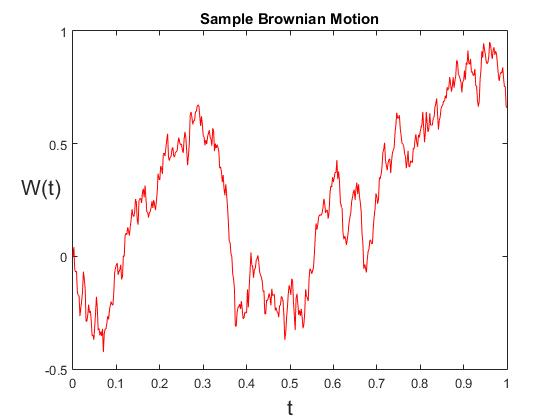
\includegraphics[scale=0.4]{example1}
		\\ \small\textbf{Fig. 1}  \textit{Discretized Brownian path from} \texttt{BPATH1.m}
	\end{center} \normalsize

	\textbf{2.2 Stochastic Integration.} Stochastic integration is required for models based on stochastic processes given the random nature of the system. This is due to the fact that deterministic integration techniques do not work. There are typically two forms of stochastic integrals, It\^{o} and Stratonovich. It\^{o} calculus is generally used as the standard for stochastic processes, however Stratonovich's integration technique has been shown to be more accurate $[5]$.\\
	\[
	\int_{0}^{T} h(t)dt = \sum_{j=0}^{N-1}h(t_j)(W(t_{j+1} - W(t_j))), \text{ It\^{o}}\]
	\[ \int_{0}^{T} h(t)dt = \sum_{j=0}^{N-1}h(\frac{t_j+t_{j+1}}{2})(W(t_{j+1}) - W(t_j)), \text{ Stratonovich}
	\]
	
	\textbf{2.3 The Euler-Maruyama Method.} The Euler-Maruyama Method is used in stochastic processes as a way to solve autonomous stochastic differential equations of the form $[2]$
	\[dX(t) = f(X(t))dt + g(X(t))dW(t) \text{, with } X(0)=X_0. \]
	However, when the Euler-Maruyama is applied to the above stochastic differential equation, the result is:
	\[dX(t) = \lambda X(t)dt + \mu X(t)dW(t) \text{, with } X(0)=X_0. \]
	This method is simply the Euler method modified to be used for stochastic differential equations. It is a generalization of the Euler's method of ordinary differential equations. The usage of the Euler-Maruyama can, however, lead to the derivation of the Black-Scholes partial differential equation $[2]$.\\
	
	\textbf{3. The Black-Scholes Partial Differential Equation Modeling System.} The point of the Black-Scholes system is to predict the value of a portfolio or assets at a point in time. In general, the asset is either a bond or a stock, the portfolio itself is comprised of both of these. There are several different methods that can be used in order to predict with the Black-Scholes. These are usually known as European and American Call Price options, both of which use geometric Brownian motion. In addition, both of these models have the same five inherent assumptions $[4]$:
	\begin{enumerate}
		\item The value of the asset can be described by geometric Brownian motion.
		\item Bonds an stocks can be bought and sold at any time since $\Delta t$ changes smoothly.
		\item $\frac{\delta V}{\delta S}$ is a smooth function and the number of stocks is allowed to vary continuously, meaning fractional shares can be bought and sold.
		\item The change in the portfolio value is due solely to change in $V$ and $S$, but it doesn't include transactional costs that are associated with the exchange of commodities.
		\item All assets can be freely bought and sold.
	\end{enumerate}
	
	\textbf{3.1 Basic Black-Scholes Model.} The Black-Scholes model can be simplified down to a very basic model for those who aren't experienced in stochastic processes or probability theory and application. This allows for the Black-Scholes to be simplified into a two equation PDE system based on the stochastic process of geometric Brownian motion and several other parameters. With the simplification of the system, there are three specific parameters become influential in the model. These parameters are stock volatility $\sigma$, stock drift $\mu$, and riskless interest rate $r$; which, in turn creates the very basic model $[4]$:
	\begin{align*}
	B_t &= e^{rt} \\
	S_t &= S_0e^{\sigma W_t + \mu t}
	\end{align*}
	
	To put the model into perspective, the parameters of riskless interest rate, stock volatility, and stock drift must be defined $[4]$. Riskless interest rate makes modeling the Black-Scholes slightly easier as $r$ represents the theoretical no loss interest rate of the stock. Stock volatility is the variation of price over time. In other words: the higher the volatility of the stock, the more likely it is to change price. The last parameter, stock drift, is the average value of the asset (stock) over time. The larger the drift, the higher the value becomes.\\
	
	This is based on martingale representation, which is based in probability and use probability distributions for defining the value of the martingale. Using filtration and measures, Martingales are usually defined as $\mathbb{P}$ or $\mathbb{Q}$ martingales. While the notation of which letter the martingale is based on is arbitrary, the measure that the letter represents is important. In the case of the Black-Scholes, martingales are used to create the Black-Scholes model's replication strategy and use the normal distribution. In doing so, the model is supposed become self-financing - meaning that once the initial value is put into the portfolio no more money is deposited into it and it sustains itself through the earnings of the stocks and bonds that can potentially increase the value of the portfolio instead maintaining a constant value.\\
	
	As the Black-Scholes depends on both stocks and bonds, the system can be hard to model due to the random nature of the stock being combined with the exponential nature of the bond. This mixes deterministic and stochastic processes for the final equation to be modeled. And while accurate, this paper's focus is on the stochastic processes that occur for the Black-Scholes. Thus, for simplicity, the bond value $B_t$ has been set at a constant of $1$ due to the self-financing property of the portfolio. Using the equation $V_t = \phi_t S_t + \psi_t B_t = E_t$, it can be found that the self-financing condition's stochastic differential equation can be solved $[4]$ and is found to be:\\
	\[S_t = e^{\sigma\hat{W}_t - \frac{\sigma^2}{2}t}\]\vspace{0.05cm}
	
	However, due to the nature of this equation being unsuitable for the modeling of the nature being based solely on the stocks over time, this stochastic differential equation was discarded in favor of the European Call Option (section 3) with simplistic Brownian motion. However, the Brownian motion chosen was not truly specified by Highman and this paper follows that of Highman's article $[2]$ by using his first code for Brownian motion (Code 1) in order to model the Black-Scholes PDE system that had been simplified to solely stock-based over time.
	\\
	
	\textbf{3.2 Non-Zero Interest Rates.} Due to the nature of the Black-Scholes, the interest rate $r$ can be zero. This is evidenced in Fig. 2, as the Black-Scholes can use Brownian motion and still be modeled with zero interest. In Fig. 2, the bond is still set to a constant value of 1 while the stocks are affected by the zero interest and Brownian motion of the stock price due to volatility and drift. To demonstrate this, the figure was run with $\sigma = 0.18$, $r=0$, $\mu=0.15$, $s_0 = 20$, and $k = 25$.
	\begin{center}
		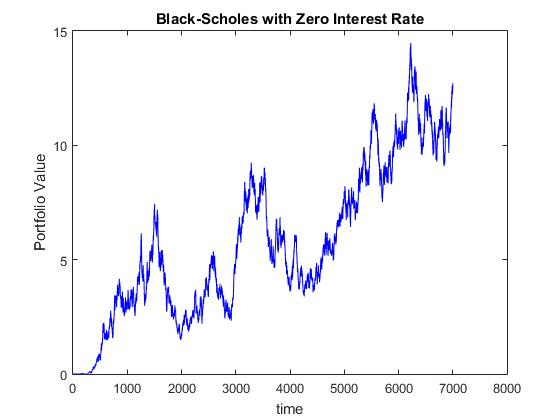
\includegraphics[scale=0.4]{zerointerest}
		\\ \textbf{Fig. 2} \textit{The Black-Scholes Using Brownian Motion with Zero Interest}
	\end{center}
	
	However, the model that zero interest rates that provides is solely a steady investment and unrealistic in markets that are both macro or micro. The non-zero interest rate cannot be ignored due to the forward contract $[4]$, which is the agreement to sell the stock for a certain price $k$ at a specified time $T$, defined as $S_T - k$. As $k$ is known to be the forward contract, a zero value at time zero leads to $k = S_0e^{rT}$ and the arbitrage to produce becomes easy to figure out. According to this rule, when $r$ was zero means that the measure for $S_t$ is not possible, thus $r \ne 0$. At a certain point, when $r \ne 0$, the growth of cash is inexorable and gets in the way of the equation. However, this can be discounted under the right conditions and non-zero interest rates were used in this paper to create a more dynamic and accurate model of the Black-Scholes.
	\\
	
	\textbf{4. The Black-Scholes Formula for European Call Price Options.} The European Call Option means that the time is set for the exchange of assets and commodities versus the American Call Option which exchanges can happen at any time. The latter is much harder to model for a beginner, thus this paper is modeling the European Call Option due to the scope of knowledge at the present time $[4]$. \\
	
	\[V(s,T) = s\Phi\Bigg(\frac{\log\frac{s}{k}+\big(r + \frac{\sigma^2}{2}\big)T}{\sigma\sqrt{T}}\Bigg) - ke^{-rT}\Phi\Bigg(\frac{\log\frac{s}{k}+\big(r - \frac{\sigma^2}{2}\big)T}{\sigma\sqrt{T}}\Bigg) \text{, where}\]
	\[ \Phi(x) = \frac{1}{\sqrt{2\pi}} \int_{-\infty}^{x} e^{-\frac{y^2}{2}}dy\]
	\\
	
	When this model is used, the value of $s$ can only be constant if the model is being used to predict the expected value of the portfolio at a specific time. This was not ideal for the paper, thus the value of $s$ was then based on geometric Brownian motion that was derived from a modified version of Code 1 $[2]$ in the appendix and Code 2 in the appendix was created using Code 1 as a base for Brownian motion to form the mathematical simulation of the Black-Scholes. This is evidenced in Fig. 3 as a simple model of the Black-Scholes was run with parameters $\sigma =0.18$, $\mu = 0.15$, $r=0.06$, $T = 7000$, $s_0 = 20$, and $k = 25$:
	\begin{center}
		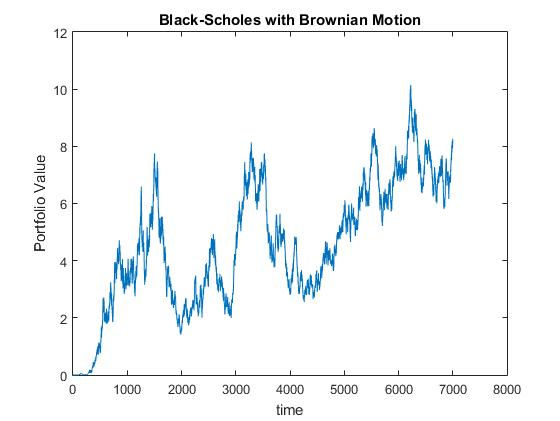
\includegraphics[scale=0.4]{example2}
		\\ \small\textbf{Fig. 3}  \textit{Sample Black-Scholes Over Time with Brownian motion}
	\end{center} \normalsize
	
	\textbf{5. Parameter Impact.} Due to multiple equations in the Black-Scholes model, there needs to be a test to see what affects the system the most. This is due to there being three parameters of note in the model - as mentioned before - that have an affect besides initial conditions and the chosen forward contract. Each of these has a different relative impact upon the model, so three models were run for each parameter separately in order to see the impact of changing the value of it while the other two were held constant. In addition to this, three more trials of five solutions were run by changing two parameters and holding the remaining one constant in order to the test and interpret the combined effect of the parameters.
	\\
	
	\textbf{5.1 Riskless Interest Rate.} The first parameter tested of the three was the riskless interest rate of the stock, $r$. The parameters of stock volatility and drift were held constant at the values $\sigma = 0.18$ and $\mu = 0.15$. This was done in order to see the impact of $r$ by itself upon the model as the parameter only appears in the Black-Scholes equation, it has no impact upon the Brownian motion of the stock.
	
	\begin{center}
		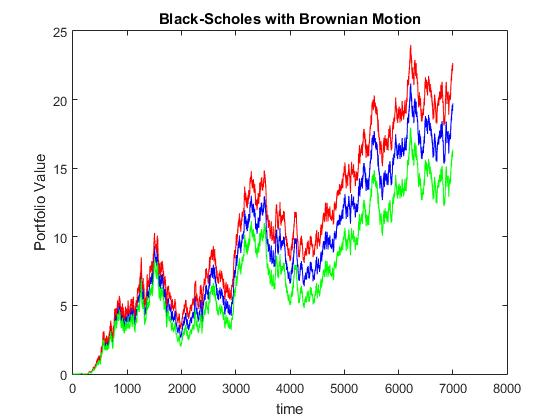
\includegraphics[scale=0.4]{interestimpact}
		\\ \textbf{Fig. 3} \textit{The Impact of Riskless Interest Rate on the Black-Scholes}
	\end{center}
	
	In Fig. 4, the original model that was run for Fig. 3 using $r = 0.06$ is imposed onto the graph in blue and is being used as a baseline to judge the effect of $r$ on the model. When the value of $r$ was increased to $r=0.09$ it was plotted on the graph in red, which was - as expected - slightly higher than that of the baseline. However, there was not a truly significant change in the expected value overall. Then the lower riskless interest rate of $r=0.03$ was run through the model and - much like the high interest rate - it also behaved as expected with the overall value of the portfolio being lower than the baseline. However, overall the riskless interest rate did not appear to have a large impact upon the value of the portfolio over time.
	\\
	
	\textbf{5.2 Stock Volatility.} The next parameter to be tested was the stock volatility, which is present in both the Brownian motion of the stock as well as in the Black-Scholes partial differential equation as well. For this, the original graph in Fig. 3 was once again graphed onto the figure in blue to serve as a baseline. For this test, the parameters of stock drift and riskless interest rate were held constant at $\mu=0.15$ and $r=0.06$.
	\begin{center}
		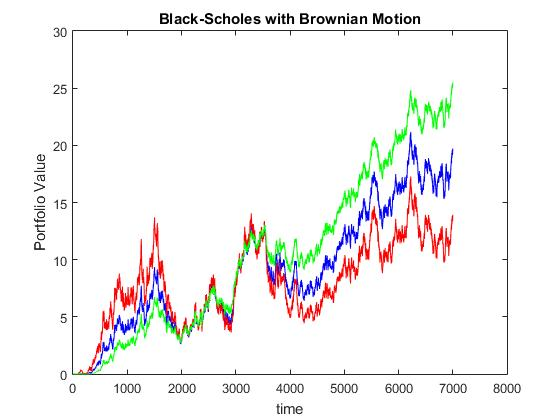
\includegraphics[scale=0.4]{voltalityimpact}
		\\ \textbf{Fig. 5} \textit{The Impact of Stock Volatility on the Black-Scholes}
	\end{center}
	
	In Fig. 5 the value of the stock volatility was changed to $\sigma = 0.27$ and $\sigma = 0.12$. These are shown with the other two parameters held constant in red and green respectively. When $\sigma$ was increased, it can be observed that the behavior of the system in the short term makes the value of the portfolio seem higher. However, the long term behavior of $\sigma$ being increased shows that the higher the stock volatility is, the less the portfolio value increases over time. When $\sigma$ is decreased the portfolio behaves the opposite with the value seeming to be lesser at the beginning, but slowly increasing over time to become a higher-valued portfolio.
	\\
	
	\textbf{5.3 Stock Drift Impact.} The last singular parameter to be tested was that of stock drift. Once again, the original simulation of the Black-Scholes was plotted on the figure in blue and the parameters $r = 0.06$ and $\sigma = 0.18$ were held constant. As this parameter appears solely in Brownian motion, the impact of its change became apparent in Fig. 6.
	\begin{center}
		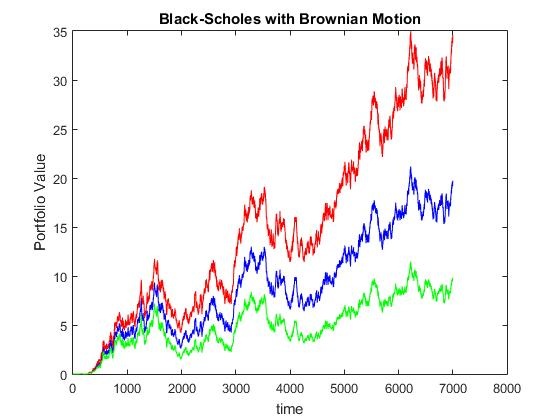
\includegraphics[scale=0.4]{driftimpact}
		\\ \textbf{Fig. 6} \textit{The Impact of Stock Drift on the Black-Scholes}
	\end{center}
	
	From Fig. 6, it can be seen that the impact of stock drift is high. When increased to $\mu  = 0.2$, the long-term value of the portfolio dramatically increases to past the desired forward contract of $k=25$. However, when decreased by the same increment of $0.05$ to $\mu = 0.1$, the value of the portfolio is impacted and is only about half of that of the original simulation. This is potentially due to the decrease cutting the value of the stock drift to 66\% of the original drift versus the increase to 133\%.
	\\
	
	\textbf{5.4 Mixed Parameter Impact.} The next step was to run three more groupings of simulations changing two parameters instead of one. The goal of this was to observe and understand the overall impact of the parameters on the Black-Scholes. As with the previous three figures, for each grouping the baseline of the simulations was kept with the original three values of the parameters being modeled in blue.
	\begin{center}
		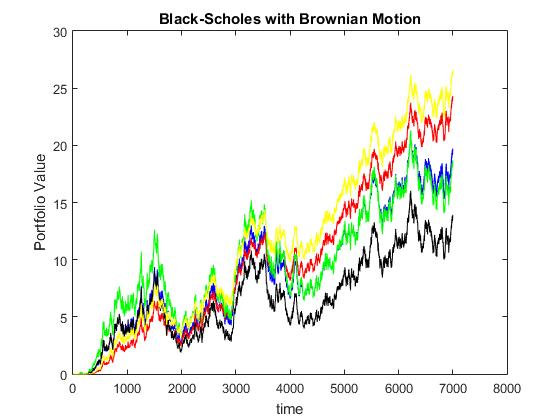
\includegraphics[scale=0.4]{ivimpact}
		\\\textbf{Fig. 7} \textit{The Mixed Impact of Stock Volatility and Riskless Interest on the Black-Scholes}
	\end{center}
	
	First, stock drift was held steady at $\mu = 0.15$ while the parameters of stock volatility and riskless interest were changed. The first test was to increase both volatility and riskless interest, setting values of $\sigma = 0.23$ and $r = 0.09$. It can be seen that the value of the portfolio is the highest with these increases at first, but ends up being similar in value to the original simulation as time goes on. Next, both parameters were decreased, setting $\sigma = 0.12$ and $r=0.05$. The behavior of the portfolio value seems to be the worst at first, but as time approaches the end of the simulation it has a much higher end value than that of the original simulation or that of the higher parameter values.
	\\
	
	From there, two more tests were implemented with one parameter being decreased while the other was increased. This was run in order to determine the behaviors of the parameters in relation to each other when they were not being affected in the same way. The first test was to increase volatility and decrease the interest rate. This was modeled in black and the value were set to $r=0.02$ and $\sigma = 0.2$. It can be seen that the value of the portfolio seems to be higher than the baseline at first, but becomes the worst value of the simulation group and results in a value lower than the baseline. The second test was to increase the interest rate and decrease the volatility. Setting the parameters to $\sigma = 0.13$ and $r=0.08$, this simulation was plotted in yellow and achieved the highest portfolio value over time.
	\begin{center}
		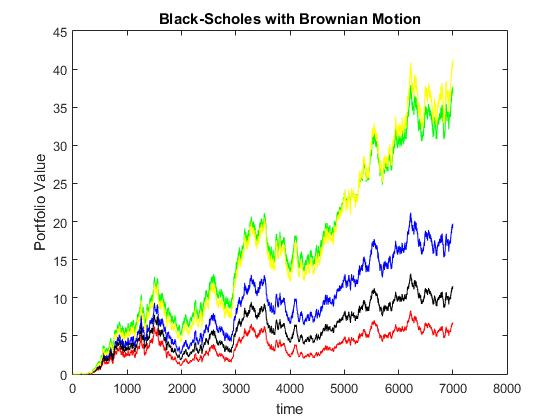
\includegraphics[scale=0.4]{idimpact}
		\\ \textbf{Fig. 8} \textit{The Mixed Impact of Stock Drift and Riskless Interest on the Black-Scholes}
	\end{center}
	
	This second grouping of simulations held the volatility stable at $\sigma = 0.18$ and changed the values riskless interest and stock drift. The first test increased both parameters, setting $r=0.09$ and $\mu =0.2$, the result was an exponentially higher portfolio value in comparison to the baseline. This is evidenced by the green simulation in Fig. 8 being larger than the blue baseline. The next test, in red, decreased both parameters, setting $\mu = 0.09$ and $r=0.04$. This resulted in the lowest portfolio value by far, at a third of the value of the baseline.\\
	
	The next step followed that of the method used before to test the parameters's relation to each other when they were not changed in the same way. The first test decreased drift and increased interest, setting $\mu = 0.1$ and $r =0.08$. This produced a low portfolio value, as evidenced by the black simulation, but it can be seen that the higher interest rate (and slightly higher drift than when both parameters were decreased) boosts the value of the portfolio slightly. The last simulation in this grouping set $\mu = 0.23$ and $r=0.02$ then plotted the result in yellow. The result is comparable to both of the parameters being increased and the higher end value of this is partially due to the drift being higher than the value set for it when both parameters were increased.
	\begin{center}
		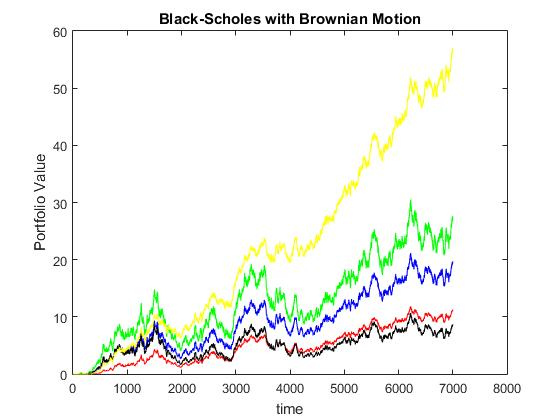
\includegraphics[scale=0.4]{vdimpact}
		\\ \textbf{Fig. 9} \textit{The Mixed Impact of Stock Drift and Volatility on the Black-Scholes}
	\end{center}
	
	This final grouping of simulations evidenced in Fig. 9 held interest rate steady at $r = 0.06$ while the parameters of stock volatility and drift were changed. The first simulation increases both volatility and drift interest, setting values of $\sigma = 0.24$ and $\mu = 0.2$. When plotted in green to compare to the baseline, this resulted in a higher portfolio value through the whole simulation in comparison to the baseline. The second test, both parameters were decreased, setting $\sigma = 0.12$ and $\mu=0.09$. The effect of these parameters both being decreased resulted in a lower portfolio value (in red) through the whole simulation.\\
	
	The last two tests for this simulation grouping were once again performed in the same manner as the prior two groupings. First, volatility was increased to $\sigma = 0.21$ and drift was decreased to $\mu=0.1$, then plotted in black. It can be seen that the value of the portfolio seems to be similar to that of the baseline at first, but becomes the worst value of the simulation group and results in a value lower than the baseline. The last simulation was plotted in yellow and increased the drift to $\mu = 0.23$ while decreasing the volatility to $0.12$. This simulation achieved the highest portfolio value over time out of all the simulation in all the groups.
	\\	
	
	\textbf{5.5 Parameter Impact Interpretation.} By holding one of the independent parameters that impacts the Black-Scholes PDE (not initial conditions), the following behaviors are observed:
	\begin{enumerate}
		\item Stock drift and interest rate have a positive correlation and relationship with each other.
		\item Stock volatility has an inverse relationship with stock drift and interest rate.
	\end{enumerate}
	
	These behaviors are interesting and evidenced in Fig. 4-9 and the impacts of each parameter is different. The stock drift, $\mu$, appears to have the most dramatic impact on the solution, this is potentially due to the fact it is only in in geometric Brownian motion and not the Black-Scholes itself. This occurs while the riskless interest rate, $r$, has the least impact on the overall behavior of the solution, perhaps due to it only playing a role in the Black-Scholes model.Finally, the stock volatility, $\sigma$ has a significant impact on the model. This could be due to its presence in both the Black-Scholes and the geometric Brownian motion.\\
	
	\textbf{5. The Linear Stability of the Black-Scholes.} The Black-Scholes equation is found to be linearly stable, this has been proven by multiple papers and is based on a popular linear boundary condition that is often applied to numerical solutions of financial partial differential equations $[6],[7]$:
	\begin{itemize}
		\item[] The second derivative of the option value, $V''$, vanishes when the underlying asset price gets large.	
	\end{itemize}
	
	This is evidenced by the maximum norm of $e^{tM}$ and $\Phi(\Delta tM)^n$ where $M$ is the matrix representing the semi-discretized Black-Scholes partial differential equation operator $\Phi$ $[6]$, defined as:
	\\
	\[ \Phi(x) = \frac{1}{\sqrt{2\pi}} \int_{-\infty}^{x} e^{-\frac{y^2}{2}}dy\]
	\vspace{0.1cm}
	
	The linear stability of the Black-Scholes results in the interpretation that growth in general has no adverse effect on convergence behavior and that the stability condition known for the constant coefficient equation should hold locally at all $S_t$.
	\\
	
	\textbf{6. The Weaknesses of the Black-Scholes.} The Black-Scholes model has many weakness, the most prominent being the five inherent assumptions it makes $[4]$. The reason these assumptions create weaknesses is due to the fact the Black-Scholes becomes invalid if any of them are violted. The weakness of the assumptions include that the asset's value can not always be described by geometric Brownian motion, time does not change smoothly with how reality's economy works, fractional shares cannot be bought and sold, transactional costs always occur, and assets cannot be freely bought and sold due to regulation. However, these are not the sole reasons that the Black-Scholes is weak. The other factors include the usage of a normal distribution, constancy of variance (or volatility), and the riskless interest rate being theoretical.
	\\
	
	\textbf{6.1 Combating the Weaknesses of the Black-Scholes.} Due to the fact that if any of the assumptions of the Black-Scholes are violated it becomes invalid and the computed option prices it simulates are not fair, the weaknesses have to be combated. To do this, geometric Brownian motion must be combated - which is not an easy task. This is due to the Brownian motion requiring that the series of first differences of log-prices must be uncorrelated, however there are small but statistically significant correlations between the differences of logs at short time lags $[8]$. There is no unified consensus among the community for what to do about this, however other ones can be mitigated.\\
	
	To start, the normal distribution can be substituted out for a leptokurtic one. The leptokurtic distribution is better for modeling a system as volatile as the Black-Scholes due to the fact that the distribution itself takes into account the commonality of outliers. Switching from a constant volatility to volatility clusters would allow for lulls and agitation in the market over time. Adding a function to create a risk for $r$ would make the model more realistic. The other factors such as transactional costs, removal of fractional shares, and the regulation of asset exchange could be added in through a multitude of functions $[8]$.\\
	
	\textbf{7. Conclusion.} The Black-Scholes model is still commonly used due to its generic capabilities. Most mathematicians who use it to model end up modifying it to make it their own and accommodate to their economies, regulations, and parameters. As a result, there's no official version of the Black-Scholes that is unanimously considered the most accurate in the community. However, the model used in this paper was purely theoretical and based on the original Black-Scholes equation. From the results, it can be seen that the parameters have varying relative influence on the equation with stock drift being the most influential and interest rate being the least. This, in turn, leads to the interpretation that the stochastic process behind the Black-Scholes is what makes it work, meaning the parameters involved in Brownian motion have th most influence.
	\newpage
	\section*{Appendix}
	\textbf{Code 1:}
	\lstinputlisting{BPATH1.m}
	\textbf{Code 2:}
	\lstinputlisting{trial.m}
	\begin{thebibliography}{20}
		\bibitem{Day}
		M. DAY, 
		A Primer on Probability and Stochastic References, 
		Unpublished (2007).
		\bibitem{Higham}
		D. J. HIGHAM, 
		An Algorithmic Introduction to Numerical Stimulation of Stochastic Differential Equation, 
		SIAM Rev., 43 (2001), 
		pp. 525-546.
		\bibitem{Scott}
		M. SCOTT, 
		Applied Stochastic Process in Science and Engineering, 
		University of Waterloo (2013), 
		pp. 2-19.
		\bibitem{Baxter}
		M. BAXTER, A. RENNIE, 
		Financial Calculus: An Introduction to Derivative Pricing, 
		Cambridge University Press (2003), 
		pp. 83-98
		\bibitem{Bichteler}
		K. BICHTELER, 
		Stochastic Integration and Stochastic Differential Equations,
		University of Texas (2010),
		pp. 43-52
		\bibitem{hout}
		K.J. HOUT, K. VOLDERS, 
		Stability and Convergence Analysis of Discretization of the Black-Scholes PDE with the Linear Boundary Condition, 
		Cornell University Library (2012), 
		pp.1-30
		\bibitem{Windcliff}
		H. WINDCLIFF, P. A. FORSYTH, K.R. VETZAL, 
		Analysis of the Stability of the Linear Boundary Condition for the Black-Scholes Equation, 
		University of Waterloo (2003), 
		pp. 2-6
		\bibitem{Privault}
		N. PRIVAULT,
		Financial Mathematics,
		Nanyang Technological University (2016)
	\end{thebibliography}
\end{document}